\documentclass{article}

\PassOptionsToPackage{numbers,compress}{natbib}
\usepackage[dblblindworkshop]{neurips_2026}
\workshoptitle{PTA: From Pretrained Representations to Acting Agents}

\usepackage[utf8]{inputenc}
\usepackage[T1]{fontenc}
\usepackage{hyperref}
\usepackage{url}
\usepackage{booktabs}
\usepackage{graphicx}
\usepackage{microtype}
\usepackage{xcolor}
\usepackage{amsmath}

\title{From Pretrained Knowledge to Action:\\
Auditing Language Models in a Deterministic Game}

\author{Anonymous Authors}

\newcommand{\bench}{\textsc{Slay-Bench}}

\begin{document}

\maketitle

\begin{abstract}
Pretrained language models can describe strategy without reliably converting that
knowledge into actions. Measuring this gap is difficult because evaluations may
confound the target capability with task semantics, interface, model authority,
response contract, and score. We present \bench, a deterministic
Slay-the-Spire-inspired simulator with four separately scored decision operations, two
characters, two state encodings, and seven open-model configurations. Differences are
operation-specific. Qwen3-235B-A22B improves fixed-deck card choice over Qwen3-32B in
all four character--encoding cells and 19/20 seed pairs, but not uniformly in immediate
sequencing, combat execution, or hybrid Act-1 rollout. Crucially, an adversarial audit
finds that always answering ``Strike'' solves all 40 removal fixtures and a deterministic
card-name dictionary solves all 120 rotated fixed-deck cases, without simulating a
transition. These tests do not show that the evaluated models used either shortcut;
they show that the instruments do not require planning. We quarantine removal, bound
fixed-deck scores as recognition and category-aligned choice, and retire the cross-task
scalar and horizon interpretation. From this completed falsification we derive a
same-state controlled-horizon protocol and a reusable audit ladder: before benchmark
scores are attributed to planning, the instrument should first survive compute-free
policies.
\end{abstract}

\section{The measurement problem}

Pretraining may encode game rules, card interactions, and strategic abstractions, yet
an acting agent must select a legal action under a concrete objective and carry its
consequences forward. PTA therefore needs measurements that distinguish \emph{stored
knowledge}, \emph{action selection}, and \emph{closed-loop control}. Existing planning
benchmarks offer exact symbolic evaluation \citep{valmeekam2023planbench}, while game
benchmarks offer interactive breadth \citep{costarelli2024gamebench,paglieri2025balrog}.
But a line drawn across heterogeneous tasks can look like a ``planning horizon'' even
when task semantics, output contracts, baselines, and agent authority all changed.

We use a deterministic deck-building game to ask a narrower question: \emph{where does
pretrained knowledge become useful for a specified decision operation?} Slay the Spire
is not new as an LLM testbed. MiniSTS studied language-driven play
\citep{bateni2024language}; subsequent work examines card-rule synergy
\citep{kim2025synergy} and original-game agents across broader suites
\citep{park2025orak}. Our contribution is an inspectable, within-simulator
\emph{operation profile} and the adversarial audit that changed its interpretation.

\paragraph{Contributions.}
First, \bench{} makes four decision operations inspectable in native units and exposes
model authority. Second, a seven-configuration profile and matched Qwen3 comparison
show operation-specific differences, including a fixed-deck card-choice gain in 4/4
cells and 19/20 seed pairs without uniform transfer. Third and centrally, a completed
adversarial audit supplies two compute-free counterexamples, retracts unsupported
scalar and horizon claims, and motivates a controlled protocol and audit ladder for
agent benchmarks.

\section{A deterministic operation profile}

\bench{} implements a deterministic, Slay-inspired simulator with independent random
streams, two characters (Ironclad and Silent), Acts 1--3 mechanics, and two semantically
matched prompt encodings: structured JSON and raw English. It is not claimed to be a
bit-exact clone of the commercial game. Table~\ref{tab:tasks} states what the model
actually controls and the construct each score can support.

\begin{table}[t]
\caption{The four operations are not levels on one horizon. ``Ref.'' is the scoring
reference; scripted choices are outside model control. Removal-v1 is quarantined.}
\label{tab:tasks}
\centering
\scriptsize
\setlength{\tabcolsep}{3.2pt}
\begin{tabular}{@{}p{1.02in}p{1.38in}p{1.08in}p{1.48in}@{}}
\toprule
Operation & Model-controlled output & Score / ref. & Supported interpretation \\
\midrule
Immediate sequence & ordered card indices for one state & damage / exhaustive best & immediate-damage sequence quality \\
Combat execution & card plays each turn & win; remaining HP / greedy bot & closed-loop combat execution \\
Fixed-deck choice & deck label; one of three cards & authored label and pick & taxonomy and card-category alignment \\
Hybrid Act-1 rollout & combat and reward choices & floors and progress / matched greedy & behavior under scripted route, rest, shop, and events \\
\bottomrule
\end{tabular}
\end{table}

The immediate oracle exhaustively enumerates legal sequences; current-code replay
completes all 200 paper-seed states below a declared 20,000-node budget (maximum 137
nodes). Combat uses a deterministic greedy reference, not optimal play. Fixed-deck
fixtures contain one authored label and one on-label card among three rotated offers.
The rollout is explicitly hybrid: the LLM chooses combat and rewards, while traversal
and several non-combat decisions are scripted. Illegal actions and parse failures score
as failures; card accuracies for unparseable outputs are not silently imputed.

\paragraph{Design and uncertainty.}
We evaluate seven configurations from five model families
\citep{dubey2024llama,jiang2023mistral,deepseek2025r1,qwen2025qwen25,yang2025qwen3} with greedy
decoding. For every available character--encoding cell, turn, combat, and fixed-deck
tasks use 20 samples at each of five base seeds $\{42,1042,2042,3042,4042\}$; their
sample streams do not overlap. Standard deviations are across base seeds. Hybrid runs
use 20 runs per seed for the balanced small-model cohort and a separately reported
5-run floor-estimate tier for Qwen3; missing cells remain missing. Format tests use
exact sign-flip permutations over matched seed pairs. With only five pairs, the minimum
two-sided per-cell $p$ is $0.0625$, so inference relies on pooled strata and paired
sample tests, not isolated null results.

\section{Results: competence is operation-specific}

Figure~\ref{fig:profile} reports native units rather than averaging non-commensurate
scores. The profile immediately rejects a one-number account. DeepSeek-R1-Distill-14B
has strong immediate sequencing but weak combat and a $-2.73$-floor hybrid result in
its one measured rollout cell. Small instruct models nearly match the greedy combat
reference while differing materially in sequencing and card choice. Hybrid progress is
usually within roughly one floor of seed-matched greedy; survival is at the same floor
(0--3\% in the balanced cohort), so we call it \emph{on par}, not a win.

\begin{figure}[t]
\centering
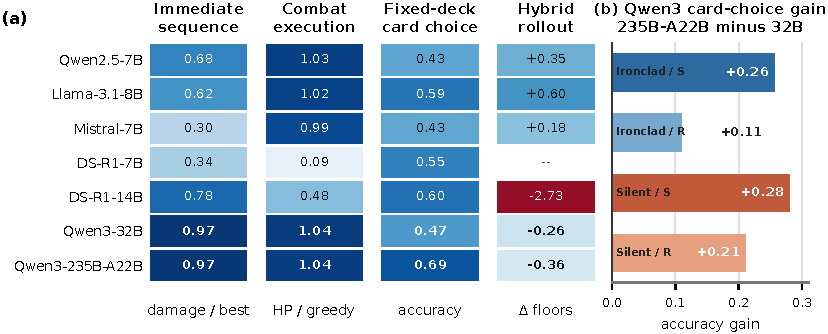
\includegraphics[width=\textwidth]{figures/operation_profile.pdf}
\caption{\textbf{Operation profiles, not a horizon curve.} (a) Each column has its own
unit and scale; entries average the four character--encoding cells when available.
Hybrid values are floors relative to a seed-matched greedy policy. DS-R1-14B hybrid is
one cell; DS-R1-7B is unmeasured. (b) Qwen3-235B-A22B minus Qwen3-32B fixed-deck
card-choice accuracy. S/R denote structured/raw. The MoE-versus-dense comparison is not
a pure scaling law.}
\label{fig:profile}
\end{figure}

\subsection{A selective Qwen3 card-choice gain}

Qwen3-235B-A22B (22B active parameters, FP8 MoE) and dense Qwen3-32B share a model
family but differ in architecture as well as nominal capacity; this is neither a pure
capacity match nor a scaling law. Card-choice gains are $+.256,+.110,+.280,+.210$ for Ironclad structured,
Ironclad raw, Silent structured, and Silent raw, respectively. Nineteen of 20 matched
seed pairs improve. Archetype recognition rises in 15 pairs, ties in three, and falls in
two. In contrast, turn differences mix signs ($+.004,+.043,-.021,-.031$), combat HP
differences mix signs, and hybrid floor differences are $-.64,-.20,-.12,+.56$.
Immediate sequencing is ceiling-limited (91--97/100 samples per cell already match the
exact oracle), but that does not manufacture the card-choice result. The defensible
conclusion is selective improvement in choosing a category-aligned card.

\subsection{Encoding changes execution, not a general capability}

Across 14 model--character strata, structured prompts improve combat win rate by
$0.0479$ (7 positive, 7 ties; pooled permutation $p=10^{-4}$) and HP ratio by $0.0593$
(12 positive, 2 negative; $p=10^{-4}$). For immediate damage, however, the pooled
magnitude favors raw by $0.0644$ while directions split 6 versus 8. Fixed-deck effects
also split by model. Thus representation format is part of the control interface, but
its sign is not a domain-general property of ``planning.''

\section{Instrument falsification: what scores cannot identify}

An instrument intended to measure planning should not award a perfect score to a
policy that never simulates a future transition. Shortcut learning is a measurement
failure when a benchmark rewards a feature that does not require the intended
capability \citep{geirhos2020shortcut}. We therefore ask the cheapest adversarial
question: \emph{what would a compute-free policy score?}

\begin{table}[t]
\caption{Instrument falsification tests and their consequences.}
\label{tab:audit}
\centering
\scriptsize
\setlength{\tabcolsep}{3.6pt}
\begin{tabular}{@{}p{1.10in}p{1.65in}p{1.00in}p{1.18in}@{}}
\toprule
Target & Degenerate policy & Result & Consequence \\
\midrule
Removal-v1 & always answer ``Strike'' & 40/40 fixtures & metric quarantined \\
Deck label + pick & card-name dictionary; choose sole on-label offer & 60/60 each; 120/120 total & bounds score as recognition \\
Cross-task scalar & reweight incomparable task units & weight-dependent & scalar and horizon curve retired \\
\bottomrule
\end{tabular}
\end{table}

Every original removal fixture has the same expert answer, \texttt{Strike}. More
subtly, each deck contains a unique signature card and each offer contains exactly one
card assigned to that label. A deterministic dictionary therefore obtains perfect
archetype and pick accuracy across 20 fixtures and three rotations per character
(60/60 each; 120/120 combined), without simulating a transition. These counterexamples
do \emph{not} show that the evaluated LLMs used either shortcut; they show that the
instruments do not \emph{require} planning. This necessity test, not the game-specific
shortcut, is reusable: a score cannot identify a capability that an excluded control
achieves perfectly. We exclude removal from every analysis and composite, rename the
surviving task fixed-deck recognition/card choice, and retire the cross-task scalar and
horizon plot.

Qwen3's observed matched-seed gain remains informative under the current labels, but it
supports category-aligned choice rather than forward search. Thus operation-specific
differences survive while the stronger planning interpretation is falsified by the
instrument itself.

\section{A controlled protocol for measuring decision horizon}

The falsification identifies the missing intervention. We specify a versioned
same-state protocol and implement its exact-search infrastructure; model evaluation
under this protocol is outside the evidence reported here. For a frozen fixture, hold
the observation, legal first actions $A$, objective $U$, response contract, simulator,
and first-action scoring fixed; vary only horizon $H\in\{1,2,4,8\}$. Exact search
assigns every legal first action an $H$-step value $q_H(a)$. The primary estimand is the
paired within-fixture change in selected-action quality from $H=1$ to $H=8$, with the
full slope reported. Model-blind fixtures must first pass three gates: their optimal
first actions change with $H$ often enough to create treatment strength; exact search
stays within an audited budget; and an $H$-mismatched policy loses on the sensitive
subset. This design changes the target construct without changing the task or interface.

\begin{figure}[h]
\centering
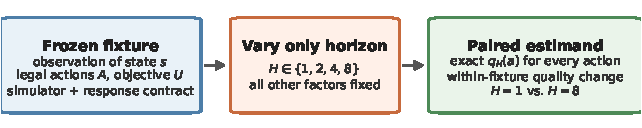
\includegraphics[width=\textwidth]{figures/controlled_h_protocol.pdf}
\caption{Controlled same-state decision-horizon protocol derived from the instrument
audit. The observation, legal actions, objective, simulator, response contract, and
first-action score remain fixed while only $H$ varies. Exact search evaluates every
legal first action. We specify the protocol here but claim no model-level horizon
result.}
\label{fig:controlled-h}
\end{figure}

\paragraph{An audit ladder for actionable-representation benchmarks.}
The completed audit suggests four gates. First, test
constant, lookup, and other compute-free policies. Second, report each operation in its
native unit with the model's authority made explicit. Third, intervene on the target
construct while freezing the state and interface. Fourth, validate authored utilities
against downstream outcomes or an external environment. \bench{} currently clears the
first two gates, specifies and implements infrastructure for the third, and does not
clear the fourth. The ladder makes evidence status legible instead of hiding it in a
scalar.

\section{Limitations and conclusion}

The simulator is deterministic but simplified and lacks conformance testing against
the original game. Fixed-deck labels and utilities are authored rather than validated
by downstream outcomes. Historical artifacts predate full provenance and run traces;
DeepSeek-7B fixed-deck accuracies are conditioned on parseable outputs. The Qwen3 run
tier has only 25 runs per cell, and the central Qwen3 comparison changes architecture as
well as capacity. Seven open configurations, two characters, and one game do not
establish general scaling or transfer. Finally, hybrid rollout does not measure a fully
autonomous agent. The model-level controlled-$H$ intervention is not evidence in this
paper, and downstream or external validation remains incomplete.

Within those limits, pretrained knowledge does not become actionable uniformly, and
apparently coherent benchmark profiles can arise from properties of the instrument
rather than forward search. Agent benchmarks should therefore be attacked with cheap
degenerate policies before their scores are interpreted as evidence of planning.
Separating decision operations, reporting native units and model authority, and
intervening on the intended construct provide a more defensible path from benchmark
performance to capability claims.

\newpage
\bibliographystyle{plainnat}
\bibliography{references}

\end{document}
